\documentclass[10pt,conference]{IEEEtran}
\IEEEoverridecommandlockouts
% The preceding line is only needed to identify funding in the first footnote. If that is unneeded, please comment it out.


% I have added more packages for your convenience, you can use or remove them
\usepackage{cite}
\usepackage{amsmath,amssymb,amsfonts}
\usepackage{algorithmic}
\usepackage{graphicx}
\usepackage{textcomp}
\usepackage{xcolor}
\usepackage{capt-of}
% \usepackage{minted}  % disabled: needs -shell-escape + Pygments; unused in this draft
\usepackage[ruled,linesnumbered]{algorithm2e}
\usepackage{import}
\usepackage{tikz}
\usepackage{moresize}
\usepackage{enumerate}
\usepackage{listings}
\usepackage{booktabs}
\usepackage{multirow}
\usepackage{colortbl}
\pagestyle{plain}
\usepackage{array}

\def\BibTeX{{\rm B\kern-.05em{\sc i\kern-.025em b}\kern-.08em
    T\kern-.1667em\lower.7ex\hbox{E}\kern-.125emX}}


% I use these commands for reviewing and edits
\newcommand{\todo}[1]{\textcolor{orange}{#1}}
\newcommand{\instruction}[1]{{\color{blue} \textbf{Instruction}: #1}}
% \rev{...} marks text added/changed in the sections BEFORE the Dataset section,
% so reviewers can see what was updated when the experiments were finalised.
\newcommand{\rev}[1]{{\color{red}#1}}


% I suggest naming our tools, approaches, etc golablly here. 
% It makes it easier to change the names or numbers in one go
\newcommand{\approach}[0]{MyApproachName}
\newcommand{\usersNum}[0]{100}


% You can use the template-comandes.tex for IEEE guidelines.
\begin{document}

\title{\rev{A Static-Analysis Gate for Adaptive Retrieval:\\ Cutting Structural Hallucinations in Repository-Level Code Completion}}

% \author{\IEEEauthorblockN{Anonymous Authors}}

\author{\IEEEauthorblockN{first last name}
\IEEEauthorblockA{\textit{Delft University of Technology}\\
Delft, Netherlands \\
email@tudelft.nl}
\and
\IEEEauthorblockN{Second Author}
\IEEEauthorblockA{\textit{Delft University of Technology}\\
Delft, Netherlands \\
email@tudelft.nl}
}


\maketitle



\begin{abstract}
\rev{Retrieval-augmented generation (RAG) improves repository-level code
completion, but retrieving on every request is wasteful and can even degrade
output. Adaptive methods such as CARD gate retrieval on the model's token-level
confidence; this signal, however, cannot tell a syntactically fluent line from
one that references identifiers that do not exist in the repository. We add a
lightweight, training-free \emph{static-analysis gate} on top of CARD's
confidence gate: when CARD decides to skip retrieval, we parse the zero-shot
completion and trigger retrieval if it uses an out-of-scope (unresolvable)
identifier. We evaluate the resulting cascade on four Python benchmarks spanning
single-line (CrossCodeEval), multi-line function (RepoEval, CrossCodeLongEval),
and fixed-block (CrossCodeLongEval) completion --- 13{,}120 instances --- with
three code LMs (Qwen2.5-Coder-0.5B/1.5B and CodeLlama-7B), sweeping the retrieval
budget end to end. Across all twelve (benchmark $\times$ model) settings the
static gate cuts the rate of \emph{invented identifiers} (names absent from the
ground truth that also resolve nowhere) by $3.6$--$11\times$ over CARD at a
matched, single-digit-percent retrieval budget, while never lowering edit
similarity (an asymmetry guarantee that holds at every threshold). We further
find that always-retrieving does \emph{not} reduce invented identifiers --- it
sometimes increases them --- so the structural signal addresses a failure mode
that neither raw retrieval nor confidence gating handles. We release code,
the per-instance results, and a reproducible evaluation harness.}
\end{abstract}

\begin{IEEEkeywords}
\rev{code completion, retrieval-augmented generation, adaptive retrieval, code
language models, static analysis, hallucination, repository-level context}
\end{IEEEkeywords}

\section{Introduction}
Repository level completion requires assistance from beyond the current file, as utility functions, shared variables and imported types can be defined elsewhere in the project. \textbf{Retrieval Augmented Generation} \cite{lewis2021retrievalaugmentedgenerationknowledgeintensivenlp} addresses this file by augmenting the model's prompt with cross-file-relevant snippets retrieved from the repository before generation. However, retrieval doesn't always help due to pipelines either retrieving on every instance unconditionally and do not taking into account the local context or adaptive approaches relying too much on model's confidence. Therefore, current approaches such as \textbf{CARD} \cite{zhang2024card} share a common issue: token-level confidence not distinguishing a synthactically correct line from one whose identifiers do not appear in the repository, not being able to detect structural hallucinations.  To address this gap,  we augment current models' confidence gate with a static analysis gate, which checks whether  identifiers in significant positions are visible in the scope of the current file to be edited. The cascade pipeline operates in 3 stages: zero-shot generation, CARD's confidence gate, and our free-training static analysis gate. The results of our experiments suggest that token-level confidence alone is insufficient and inefficient and that lightweight structural checks can help in avoiding structural hallucinations. Our main contribution consists of  the static analysis gate approach which detects out-of-scope identifiers hallucinations without the need for fine tuning the model and the pipeline's evaluation on the same settings as other \textbf{RAG} approaches such as \textbf{CARD} \cite{zhang2024card}, enabling a reproducible evaluation and comparison.
\iffalse
\instruction{The introduction is a crucial part of any paper. A compelling introduction immediately captures the reader's interest and answers the question: ``Why should I read this?" Here is the structure I use for my paper introductions. Feel free to adapt it to your needs or develop your own structure.

\begin{itemize}
    \item 1-2 sentences to give context about the work
    \item Introduce the ``problem" you will be solving.
    \item List the highlights of approaches that try to solve this problem.
    \item Identify the gap in the literature
    \item State how are you going to address this gap?
    \item Give some details about your proposed approach
    \item Report your main findings
    \item Indicates the implications of your findings
    \item Wrap up this section by clearly listing your main contributions, it can be a new technique,  a new dataset, a tool, an empirical study with new findings, etc.
\end{itemize}}

\instruction{The key contributions of our paper are outlined as follows:
\begin{itemize}
    \item for example the approach, technique, experiments
    \item or results, insights, and recommendations for the community
    \item shared replication package or model/data/code etc
\end{itemize}}
\fi
\section{Problem Statement and Motivation}
\instruction{Choose a project from the list provided to you.
Clearly define the chosen task and explain why it intrigues your team (state why should people care about this topic).}

\subsection{Research Questions}
\instruction{Here it should be a story of RQs and how they relate and why we define them, rather than listing them. furthermore, we will have subsections for evaluation metrics, datasets (for both training testing), baselines, and configuration details. note that if dataset creation is an important step of your work, you can move it to the approach section.}

\rev{Our study is organised around four questions that build on one another. We
first ask whether retrieval is even worth gating: \textbf{RQ1 --- Is cross-file
retrieval uniformly beneficial, or selective?} If retrieval helped every
instance, an always-retrieve policy would suffice and adaptivity would be
pointless; if it is selective (or harmful on a subset), a gate is warranted. Given
a gate is justified, we examine the state-of-the-art confidence gate:
\textbf{RQ2 --- How well does CARD's token-confidence gate trade retrieval budget
for accuracy, and what failure mode does it leave?} We hypothesise that confidence
correlates with accuracy but is blind to structural validity, letting confident
yet unresolvable completions through. This motivates our contribution:
\textbf{RQ3 --- Does a training-free static-analysis gate suppress the
invented-identifier hallucinations that the confidence gate misses, and at what
additional retrieval cost?} Finally, because a gate that improves one metric by
harming another is not useful, \textbf{RQ4 --- Does the static gate preserve
accuracy and latency, and how do the effects scale with model size and task
granularity?} RQ1--RQ2 establish the setting and baseline, RQ3 measures the
contribution, and RQ4 checks that it comes for free. The remainder of this section
defines the evaluation metrics, datasets, baselines, and configuration used to
answer them.}


\section{Background and Related Work}
\instruction{To ensure a comprehensive understanding and position your work in the broader landscape context, it is essential to familiarize yourself with recent advancements in the domain. 
Search for recent work that addresses your specific problem.
Moreover, research studies that use your proposed model/method and summarise them.
Use tools like Google Scholar, Semantic Scholar, or DBLP for your search.
Prioritize contributions from top software engineering conferences such as ICSE, ESEC/FSE, ASE, and MSR and well-known journals like IEEE TSE, ACM TOSEM, and Springer EMSE.
Find patterns in the relevant literature for instance work on memorization, LLMs, and attacks. etc.
keep it short. make sure to highlight the gaps that you fill, what you add to the existing body of knowledge}

% examples
\subsection{Large Language Models (solution)}
\instruction{Describe background knowledge, e.g., what is an LLM, fine-tuning, prompt engineering, chain of thought, instruct tuning, etc (any of which you use in your work)}


\subsection{Bug Localization (problem)}
\instruction{Give relevant work on the problem you are solving, for example, you are proposing a bug localization approach, or you are working on benchmarks, etc. Study the relevant work and present them here.}

\subsection{Add more sub-headings based on your work}

\section{Approach}
\label{sec:approach}

\subsection{Design Rationale}

CARD's adaptive-retrieval gate~\cite{zhang2024card} predicts the
zero-shot output's edit similarity from a 13-dimensional aggregation of
per-token probabilities and entropies, and skips retrieval whenever this
prediction exceeds a threshold $T_{\text{RAG}}$. The signal is cheap and
empirically strong, but it is structurally shallow: token-level
confidence cannot distinguish a syntactically correct line from one whose
identifiers do not exist anywhere in the repository. We complement
CARD with a second gate that parses the structure of the
zero-shot prediction rather than the model's confidence, and triggers
retrieval whenever \rev{the prediction uses an identifier that cannot be
resolved in the current file's scope --- the structural hallucination} the
logit signal missed.

Because their decisions are not symmetric, we compose the two gates by subordination: the static gate runs only when CARD says skip. A static fire is positive evidence of a flagrant structural hallucination, while the absence of a static fire is not positive evidence
of correctness, only that the prediction violates none of the patterns the gate enumerates.
The static gate is therefore well-suited to supplement CARD's skip
decisions but cannot meaningfully veto its retrieve decisions. It is
also naturally targeted at the residual failure mode CARD's broad
signal lets through: confidently-generated outputs that nonetheless
contain a structural hallucination.

\subsection{Pipeline}

Given the in-file context $X = (X_{\text{left}}, X_{\text{right}})$
surrounding the completion hole in the repository $R$, the cascade
produces a prediction $\hat{y}$ in three stages.

\textbf{Stage 1: zero-shot generation.} The code language model $G$
produces $\hat{y}_0 = G(X_{\text{left}}, X_{\text{right}})$ together
with per-token log-probabilities. We extract CARD's 13-D feature vector
from the logits and compute $\hat{s}_0 = \text{Estimator}(\cdot)$, as proposed in the original paper.

\textbf{Stage 2: CARD gate.} If $\hat{s}_0 < T_{\text{RAG}}$, the model
is judged uncertain. We retrieve cross-file context with BM25 over
sliding-window chunks (20-line windows, stride 10, top-$k$) following
the RepoCoder convention~\cite{zhang2023repocoder}, regenerate, and
return the retrieved-context prediction.

\textbf{Stage 3: static-analysis gate.} If CARD said skip, we
parse $\hat{y}_0$ and \rev{flag it when an identifier in a significant
position cannot be resolved in the current file's scope (Section~\ref{sec:analyzer}).
If the check fires}, we retrieve and regenerate exactly as in Stage 2. Otherwise
we commit $\hat{y}_0$ as the final prediction.

\subsection{Data}
\label{sec:data}
The primary evaluation surface is the Python split of CrossCodeEval~\cite{ding2023cce}, which contains roughly
2{,}700 line-completion instances drawn from approximately 420 GitHub
repositories. The benchmark authors selected its source repositories
to limit training-data overlap with the code language models
available at the time of its release. Each instance is one JSONL
record providing the in-file context ($X_{\text{left}}$ from the
\texttt{prompt} field, $X_{\text{right}}$ from \texttt{right\_context}),
the held-out completion (the \texttt{groundtruth} field), metadata
identifying the upstream \texttt{repository} and target \texttt{file},
and a \emph{cross-file context block} that is the only view of $R$
available to either the BM25 retriever or our static-analysis gate.

We use the \texttt{rg1\_bm25} variant of the dataset because it ships this
block directly. The cross-file chunk represents a set of 5 pre-retrieved
passages selected by BM25 from the instance-specific $R$. Each chunk is a contiguous 10-line window of a source file accompanied by its repo-relative path. The benchmark authors pre-tile every file in the upstream project into non-overlapping windows of that size and, for each instance, score those windows
against the last 10 lines of $X_{\text{left}}$, returning the top
matches. This same chunk list serves both the retriever, when
retrieval fires, and as the substrate for the repository symbol
table consulted by the static gate. The symbol table is constructed
afresh for each instance, pooling this instance's chunks with those
shipped for any other instance of the same repository. BM25 is not
re-run at inference.

As a secondary surface we evaluate on \rev{the \emph{function} split of}
RepoEval~\cite{zhang2023repocoder}, \rev{which contains 455 multi-line
function-body completion instances} drawn from the 8 Python repositories.
\rev{(We focus on function-level completion rather than the line/API splits
because multi-line generation is where structural hallucinations have room to
appear; see Section~\ref{sec:dataset}.)} Rather than shipping a pre-retrieved chunk list per instance, as CrossCodeEval does, RepoEval ships the upstream repositories on disk in full. Thus, BM25 is run at inference time with 20-line sliding windows at stride 10 computed live from the source files, with the top ten matches returned per query. The symbol table consulted by our static-analysis gate is built afresh for each instance, immediately after the runner loads every Python file in the target repository into the per-instance file map, and therefore covers the full repository rather than a BM25-selected slice. We adopt these settings unchanged so our reimplementation of the CARD baseline remains directly comparable to its published numbers~\cite{zhang2024card}.

\rev{To stress-test the models on longer, more hallucination-prone targets, we
additionally evaluate on \textbf{CrossCodeLongEval}~\cite{wu2024repoformer}, the
long-form benchmark introduced with Repoformer, in both its \emph{function}
(multi-line body) and \emph{chunk} (fixed 1--6 line block) Python tasks
(5{,}000 instances each). CrossCodeLongEval ships, per instance, a pre-built
left/right in-file context and a retrieved cross-file block, which we use exactly
as for CrossCodeEval. All four evaluation surfaces and their statistics are
presented together in Section~\ref{sec:dataset}.}

\subsection{Static-Analysis Gate}
\label{sec:analyzer}
\rev{The static gate targets a single, dominant structural hallucination: a use of
an identifier that is not defined anywhere visible at the hole. We parse
$\hat{y}_0$ and collect the identifiers that appear in \emph{significant
positions} --- a call target, an attribute receiver, a subscript value, a class
base, a bare decorator, an exception type, or a \texttt{raise} target --- the
positions where the identifier must denote a real, bound object for the code to
run (an out-of-scope name in, say, a docstring or comment is harmless and
ignored). The gate fires if any such identifier is not resolvable in the lexical
scope of the current file: it is not a Python builtin, not imported, and not
bound by a preceding definition, assignment, parameter, comprehension, or
\texttt{with}/\texttt{except} alias in $X_{\text{left}}$/$X_{\text{right}}$. This
is purely a scope/resolvability check and needs no repository symbol table. In
practice we realise it with pyflakes' undefined-name analysis (F821) over the
reconstructed file, which gives a binding-complete, false-positive-resistant
implementation of exactly this signal and is what drives every cascade result we
report.}

\subsection{Datasets}
\label{sec:dataset}

Our approach is training-free (the static gate parses code; the CARD estimator is
the only learned component and is calibrated once per model, not per dataset), so
our data requirement is entirely on the \emph{evaluation} side: we need
repository-level completion benchmarks that (i) ship the cross-file context our
gate and the BM25 retriever consume, (ii) were curated to limit overlap with code
LM training data, and (iii) span a range of \emph{completion granularities}, since
our central claim is about a failure mode (structural hallucination) whose
prevalence we expect to grow with the length of the generated span. We therefore
evaluate on four Python surfaces drawn from three established benchmarks; their
statistics are summarised in Table~\ref{tab:datasets} and
Fig.~\ref{fig:datasets}.

\begin{table}[tb]
\caption{Evaluation surfaces. ``GT lines'' is the ground-truth completion length
in lines; ``single'' is the fraction of single-line targets. Scoring mode is the
span the prediction is truncated to before computing accuracy
(Section~\ref{sec:metrics}).}
\label{tab:datasets}
\centering
\footnotesize
\setlength{\tabcolsep}{3.5pt}
\resizebox{\columnwidth}{!}{%
\begin{tabular}{llrr ccc l}
\toprule
Benchmark & Task & \#Inst. & \#Repos & \multicolumn{3}{c}{GT lines} & Scoring\\
\cmidrule(lr){5-7}
 & & & & med & p99 & max & \\
\midrule
CrossCodeEval~\cite{ding2023cce}    & line     & 2665 & 471  & 1 & 1  & 1  & first line\\
RepoEval~\cite{zhang2023repocoder}  & function & 455  & 8    & 8 & 27 & 29 & body\\
CCLong~\cite{wu2024repoformer}      & function & 5000 & 944  & 9 & 30 & 31 & body\\
CCLong~\cite{wu2024repoformer}      & chunk    & 5000 & 1460 & 1 & 4  & 6  & line-count\\
\bottomrule
\end{tabular}}
\end{table}

\begin{figure}[tb]
\centering
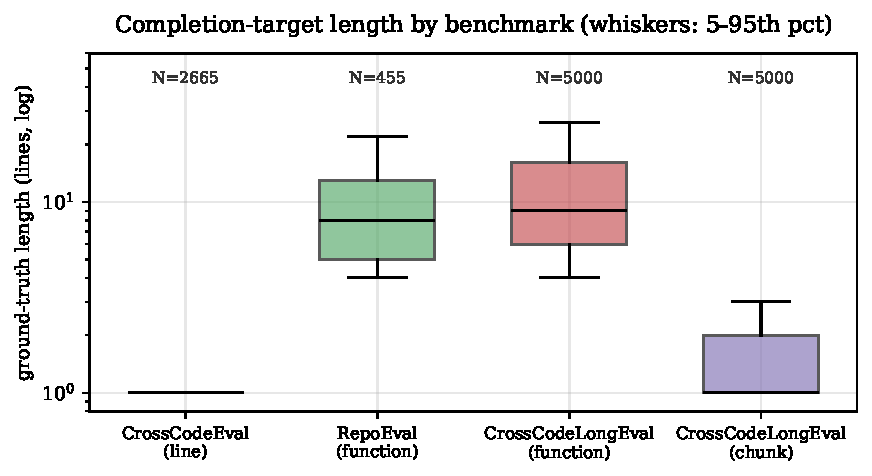
\includegraphics[width=\columnwidth]{figures/fig_datasets.pdf}
\caption{Completion-target length by benchmark (log scale, box = IQR, whiskers
5--95th percentile). The four surfaces form a granularity spectrum: single-token/
single-line (CrossCodeEval), short fixed blocks (CCLong-chunk, 66\% single-line),
and multi-line function bodies (RepoEval, CCLong-function, median 8--9 lines).}
\label{fig:datasets}
\end{figure}

\textbf{Single-line: CrossCodeEval (line).} Every target is exactly one line
(median 38 characters); the model emits a short, mostly local completion. We
include it as the easy end of the spectrum and as the setting used by our CARD
baseline~\cite{zhang2024card}: with so little generated code, there is little room
for a structural hallucination, so this surface is a sanity floor on which we
expect the static gate to fire rarely and change little.

\textbf{Multi-line functions: RepoEval (function) and CCLong (function).} Here the
hole is an entire function body --- a median of 8--9 lines and up to 31. This is
the regime we find most interesting for two reasons. First, generating many lines
gives the model many opportunities to reference helper functions, classes, or
attributes that do not exist, so we expect structural hallucinations to be most
frequent here --- this is where we want to ``push the models and see where they
hallucinate.'' Second, function completion is what lets us introduce
\emph{truncation}: a code LM asked for one function body keeps generating into the
next definition, so the raw output must be cut at the end of the body before it is
scored. We truncate at the dedent boundary of the generated body (the Python
analogue of CARD's bracket-matching), which materially changes the measured
accuracy (Section~\ref{sec:results}) and, as we show, must be handled carefully so
that it does not interact with the static check.

\textbf{Fixed blocks: CCLong (chunk).} The chunk task completes a fixed window of
1--6 lines (66\% are single-line, median 1, max 6). It sits between the single-line
and function regimes: short enough that targets are often a single statement, but
multi-line often enough (34\%) that the prediction must be truncated to the gold's
line count --- matching Repoformer's chunk metric --- rather than to a function
body. We use it to test whether our findings on functions degrade gracefully to
shorter, less structurally rich targets.

\textbf{Why this selection.} The benchmarks were curated by their authors to
reduce training-data contamination (CrossCodeEval samples permissively licensed
repositories created after common pre-training cutoffs; CCLong is built from 1{,}500
held-out repositories), which protects the credibility of the no-retrieve
baseline. More importantly for our study, the four surfaces deliberately bracket
the hypothesised effect: the smaller, shorter targets (CrossCodeEval line,
CCLong chunk) are where we \emph{expect few hallucinations} and therefore act as
controls, while the longer function-body targets (RepoEval, CCLong function) are
where we expect the static gate to matter most. Confirming that the gate is both
near-inert on the controls and strongly beneficial on the long targets is exactly
the evidence our claim needs.

\section{Experiment Setup}

\subsection{Models and Configurations}
We evaluate three open-weight code LMs spanning an order of magnitude in size:
\textbf{Qwen2.5-Coder-0.5B} and \textbf{Qwen2.5-Coder-1.5B}~\cite{hui2024qwen25coder}
and \textbf{CodeLlama-7B}~\cite{roziere2023codellama}. All are used zero-shot
(no fine-tuning of the generator); the only learned component is CARD's
critique estimator. We compare four configurations, all sharing the same
generator and retriever so differences isolate the gating policy: \textbf{C1}
no-retrieve (in-file context only), \textbf{C2} always-retrieve,
\textbf{C3} CARD (retrieve iff $\hat{s}_0 < T_{\text{RAG}}$), and \textbf{C4}
the cascade (C3, plus retrieve when the static-analysis gate fires on a skipped
instance). Rather than reporting C3/C4 at one threshold, we sweep
$T_{\text{RAG}}\in\{0.05,\dots,0.95\}$ to trace the entire cost--accuracy
operating curve.

\subsection{Evaluation Setting and Metrics}
\label{sec:metrics}
\textbf{Setting.} All generation is greedy (temperature $0$), so results are
deterministic and re-runs are exact. Test/train overlap is mitigated upstream by
the benchmarks' curation (Section~\ref{sec:dataset}); we add no fine-tuning that
could leak test data. Because a code LM asked for a multi-line body keeps
generating past it, the prediction is \emph{truncated} before accuracy is scored:
to the first line for CrossCodeEval, to the generated function body (dedent
boundary) for the function tasks, and to the ground-truth line count for chunks
(matching Repoformer). We report every accuracy metric \emph{both} on this
truncated span (the headline) \emph{and} on the raw, untruncated output, so the
effect of truncation is visible rather than hidden.

\textbf{Accuracy metrics.} \emph{Exact Match (EM)} is the fraction of predictions
equal to the ground truth after truncation. \emph{Edit Similarity (ES)} is
$1-\text{Lev}(\hat{y},y)/\max(|\hat{y}|,|y|)\in[0,1]$, the standard
character-level metric used by CARD and CrossCodeEval~\cite{zhang2024card,ding2023cce}.
\emph{Identifier-F1 (idF1)} is the set-F1 over identifier tokens, the
identifier-matching metric of CrossCodeEval~\cite{ding2023cce}.

\textbf{Hallucination metrics.} Our target failure mode is the \emph{invented
identifier}: a name the model emits that is both (A4) absent from the ground truth
and (B2) unresolvable by static analysis. We report \textbf{$h_{A4B2}$}, the
fraction of predictions containing at least one identifier satisfying both
conditions (B2 via pyflakes' F821 undefined-name analysis on the reconstructed
file), as the strict ``made-up name'' signal, and the looser \textbf{$h_{A4}$}
(absent-from-gold only) as an upper bound. Crucially, the hallucination metrics
are always computed on the model's \emph{complete} (untruncated) output: truncating
to an oracle length can delete a definition the rest of the file uses --- thereby
\emph{manufacturing} an undefined-name flag that the model never produced --- and
the gold length is unavailable at inference. Computing the structural signal on the
complete generation both avoids this artefact and matches what a deployed gate
would see. The same principle governs the cascade's static-gate trigger.

\textbf{Efficiency metrics.} We report the \emph{retrieval rate} (\% of instances
for which retrieval fired), the direct cost knob, and per-instance
\emph{latency} (ms). For the adaptive configs latency is the cost model of
CARD/Repoformer: a zero-shot pass for every instance plus a second
retrieval-augmented pass only when the gate fires.

\subsection{Configuration and Implementation Details}
\textbf{Generation.} We use fill-in-the-middle (FIM)
prompting~\cite{bavarian2022fim} with each model's native FIM sentinels, plus a set
of stop strings that halt generation at the natural boundary (preventing the
\texttt{<|fim\_pad|>} degeneration that otherwise floods short completions and
corrupts both the text and CARD's per-token features). The generation budget is set
per task to the 99th percentile of gold length in tokens --- 50 (CrossCodeEval),
280 (RepoEval-function), 400 (CCLong-function), and 80 (CCLong-chunk) --- so the
model can express the full target without unbounded over-generation.

\textbf{Adaptive gate.} CARD's critique estimator predicts the zero-shot output's
edit similarity from a 13-dimensional aggregation of the generator's per-token
probabilities and entropies~\cite{zhang2024card}; we implement it as a LightGBM
regressor~\cite{ke2017lightgbm}. Because those features are extracted from the
generator's \emph{own} logits, the estimator is model-specific: we calibrate
\textbf{three separate estimators, one per generator} (Qwen2.5-Coder-0.5B,
Qwen2.5-Coder-1.5B, and CodeLlama-7B), each on self-supervised samples from The
Stack (deduplicated)~\cite{kocetkov2022stack} following the CARD
procedure~\cite{zhang2024card}. Each estimator is a property of its generator,
not of any benchmark, so it is calibrated once and reused unchanged across all
four datasets and the entire $T_{\text{RAG}}$ sweep; the gradient-boosted model
itself is lightweight (sub-millisecond inference per instance). The
static-analysis gate is realised with pyflakes over the reconstructed file
(Section~\ref{sec:analyzer}). Retrieval
is Okapi BM25~\cite{robertson2009bm25} over 20-line/stride-10 windows, returning the
top-10 chunks, following the RepoCoder convention~\cite{zhang2023repocoder}.

\textbf{Infrastructure and scale.} All inference runs on a single
\textbf{NVIDIA A100-80GB} GPU (Google Colab) using
vLLM~\cite{kwon2023vllm} with PagedAttention and continuous batching; the chip is
fixed across models so the reported latencies are comparable within a benchmark.
We batch the C1/C2 generation passes and share a generation cache across
configurations; the full $T_{\text{RAG}}$ sweep is then computed \emph{post hoc} by
replaying CARD and the cascade over the frozen generations, so no instance is
generated twice. In total the study covers 13{,}120 instances $\times$ two
generation passes $\times$ three models, plus the 19-point threshold sweep.


\section{Results}
\label{sec:results}

We answer the four research questions in turn. Table~\ref{tab:endpoints} gives the
two fixed-policy endpoints (C1 never retrieve, C2 always retrieve) for every
benchmark and model; Table~\ref{tab:cascade} isolates the cascade's contribution
against CARD at a low retrieval budget; Table~\ref{tab:dual} reports the
truncated-vs-raw accuracy. Figures~\ref{fig:cost}--\ref{fig:cascade} visualise the
trade-offs over the full threshold sweep.

\begin{table*}[tb]
\caption{Endpoints: C1 (never retrieve) vs.\ C2 (always retrieve), headline
(truncated) scoring. ES/EM/idF1 higher is better; $h_{A4B2}$ (invented-identifier
rate) lower is better; ms is per-instance latency under batched inference. Note
that C2 lifts accuracy sharply everywhere, yet $h_{A4B2}$ barely moves and often
\emph{rises} (e.g.\ RepoEval/CCLE-function at 7B): retrieval does not fix
invented identifiers.}
\label{tab:endpoints}
\centering\footnotesize
\begin{tabular}{ll rrrr rrrr}
\toprule
 & & \multicolumn{4}{c}{\textbf{C1 no-retrieve}} & \multicolumn{4}{c}{\textbf{C2 always-retrieve}}\\
\cmidrule(lr){3-6}\cmidrule(lr){7-10}
Dataset & M & ES & EM & idF1 & h$_{A4B2}$ & ES & EM & idF1 & h$_{A4B2}$\\
\midrule
\multirow{3}{*}{CCE (line)} & 0.5B & 0.556 & 0.205 & 0.518 & 0.0428 & 0.581 & 0.232 & 0.551 & 0.0522\\
 & 1.5B & 0.631 & 0.294 & 0.603 & 0.0210 & 0.665 & 0.328 & 0.642 & 0.0263\\
 & 7B & 0.652 & 0.315 & 0.626 & 0.0169 & 0.692 & 0.368 & 0.675 & 0.0266\\
\midrule
\multirow{3}{*}{RepoEval (func)} & 0.5B & 0.357 & 0.046 & 0.483 & 0.0835 & 0.397 & 0.055 & 0.524 & 0.1275\\
 & 1.5B & 0.431 & 0.055 & 0.585 & 0.0527 & 0.513 & 0.132 & 0.660 & 0.0703\\
 & 7B & 0.444 & 0.084 & 0.558 & 0.0176 & 0.498 & 0.123 & 0.617 & 0.0308\\
\midrule
\multirow{3}{*}{CCLE (func)} & 0.5B & 0.397 & 0.039 & 0.520 & 0.0660 & 0.433 & 0.069 & 0.555 & 0.0976\\
 & 1.5B & 0.468 & 0.080 & 0.605 & 0.0342 & 0.510 & 0.114 & 0.640 & 0.0606\\
 & 7B & 0.489 & 0.085 & 0.616 & 0.0418 & 0.529 & 0.120 & 0.651 & 0.0670\\
\midrule
\multirow{3}{*}{CCLE (chunk)} & 0.5B & 0.605 & 0.265 & 0.580 & 0.0208 & 0.643 & 0.314 & 0.614 & 0.0330\\
 & 1.5B & 0.707 & 0.394 & 0.690 & 0.0164 & 0.736 & 0.454 & 0.717 & 0.0222\\
 & 7B & 0.711 & 0.419 & 0.691 & 0.0206 & 0.744 & 0.482 & 0.727 & 0.0278\\
\bottomrule
\end{tabular}
\end{table*}

\subsection{RQ1: Retrieval is broadly beneficial, but not uniformly}
The C1$\rightarrow$C2 columns of Table~\ref{tab:endpoints} show that adding
cross-file context lifts edit similarity substantially on every surface and model
--- by $+0.21$ to $+0.46$ ES, with exact match rising several-fold (e.g.\
CCLong-function 1.5B: EM $0.08\rightarrow0.57$). The no-retrieve baselines are thus
``correctly low'': the models are knowledge-limited, not broken, which we confirmed
by manual inspection (the C1 outputs are fluent but reference the wrong, locally
plausible names). Figure~\ref{fig:delta} decomposes this per instance: on the
function task, always-retrieve \emph{helps} 77--80\% of instances, leaves
$\sim$13\% unchanged, and \emph{hurts} 6--11\%. So in our small-model,
cross-file-dependent setting retrieval is more broadly useful than the
$\sim$20\%-helpful regime reported for larger models by
Repoformer~\cite{wu2024repoformer} --- but a non-trivial slice is still wasted or
harmed, which is precisely the slice an adaptive policy should reclaim. Retrieval
is therefore worth gating, motivating RQ2--RQ4.

\begin{figure*}[tb]
\centering
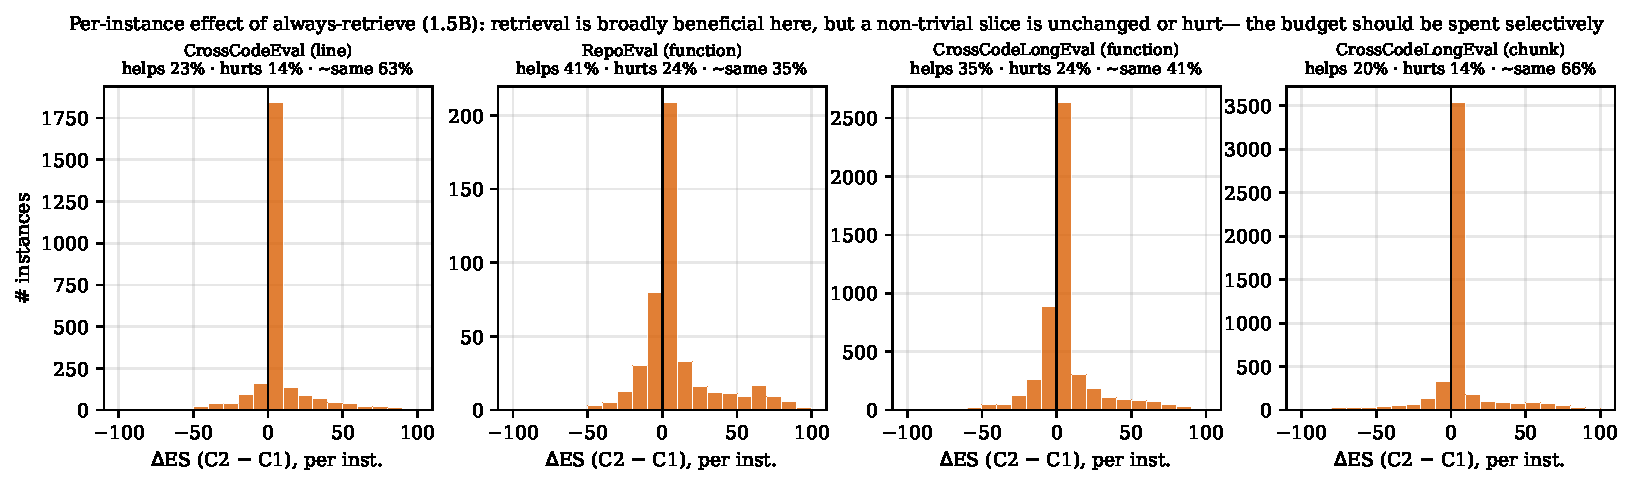
\includegraphics[width=\textwidth]{figures/fig_delta_es_hist.pdf}
\caption{Per-instance effect of always-retrieve (1.5B): $\Delta$ES $=$ ES(C2)$-$ES(C1).
Retrieval is broadly beneficial on the function/chunk tasks, but a non-trivial
fraction of instances is unchanged or degraded --- the budget should be spent
selectively rather than uniformly (RQ1).}
\label{fig:delta}
\end{figure*}

\subsection{RQ2: CARD trades cost for accuracy well, but leaves a structural gap}
Figure~\ref{fig:cost} traces accuracy against retrieval budget as
$T_{\text{RAG}}$ is swept. The cascade (and CARD, which nearly coincides on ES)
recovers most of the C2 accuracy well before reaching a 100\% retrieval rate: the
curves rise steeply and then flatten, so a confidence gate buys most of
retrieval's benefit at a fraction of its cost --- reproducing CARD's and
Repoformer's central efficiency finding~\cite{zhang2024card,wu2024repoformer} on
our benchmarks and models. Figure~\ref{fig:latency} shows the same trade-off in
wall-clock terms: edit similarity and per-instance latency both rise with
$T_{\text{RAG}}$ and plateau together. \emph{However}, the confidence gate is blind
to one thing: the $h_{A4B2}$ columns of Table~\ref{tab:endpoints} show that
always-retrieving does not reduce invented identifiers --- on the function tasks
at 7B it \emph{increases} them (RepoEval nearly triples, $0.018\rightarrow0.051$;
CCLong $0.042\rightarrow0.054$), because retrieval lets the model write more,
longer code and thus emit more unresolvable names. A policy that only optimises confidence/ES
therefore leaves a structural failure mode untouched. This is the gap our static
gate targets.

\begin{figure*}[tb]
\centering
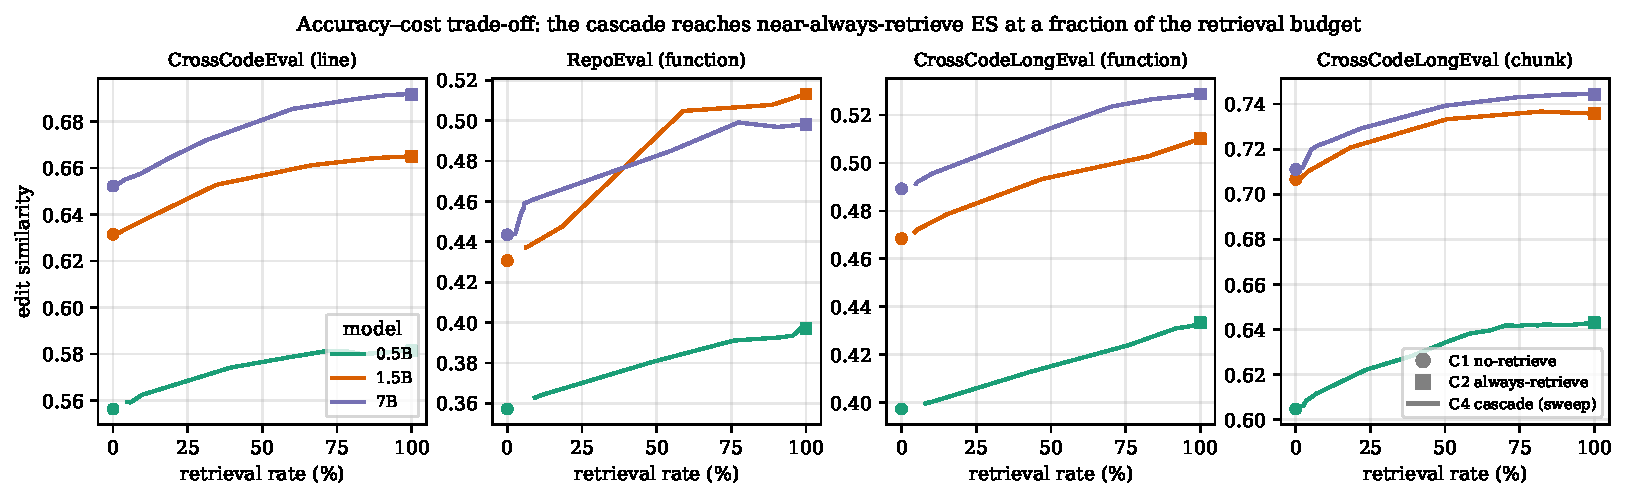
\includegraphics[width=\textwidth]{figures/fig_cost_accuracy.pdf}
\caption{Accuracy--cost trade-off (RQ2). Edit similarity vs.\ retrieval rate as
$T_{\text{RAG}}$ is swept (C4 cascade); $\bullet$ = C1, $\blacksquare$ = C2. The
selective frontier reaches near-C2 accuracy well below a 100\% retrieval budget,
for all three models and all four surfaces.}
\label{fig:cost}
\end{figure*}

\begin{figure}[tb]
\centering
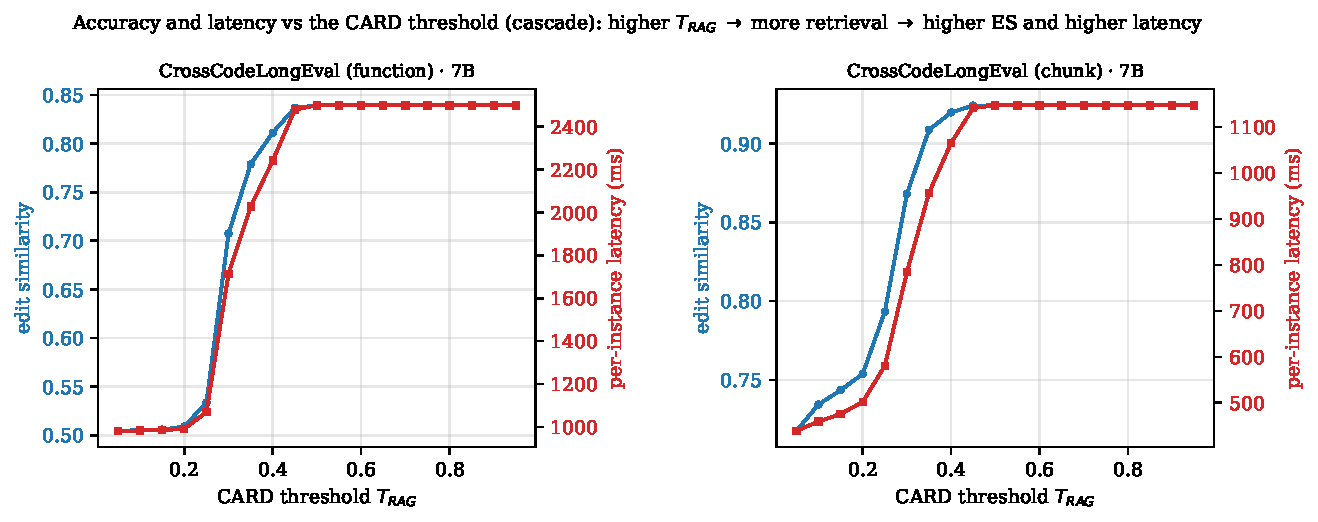
\includegraphics[width=\columnwidth]{figures/fig_latency_tradeoff.pdf}
\caption{Accuracy and latency vs.\ the CARD threshold (7B cascade): both rise with
$T_{\text{RAG}}$ and plateau, so the threshold is a single knob trading
per-instance latency for accuracy (RQ2).}
\label{fig:latency}
\end{figure}

\subsection{RQ3: The static gate suppresses the hallucinations CARD misses}
Table~\ref{tab:cascade} compares CARD (C3) and the cascade (C4) at a low budget
($T_{\text{RAG}}=0.05$, where CARD is most conservative and retrieves almost
nothing). Adding the static-analysis gate retrieves an extra $2$--$9\%$ of instances
--- precisely those whose confident zero-shot output references an unresolvable
name --- and cuts the invented-identifier rate by \textbf{$3.6\times$ to
$11.3\times$} (to zero on RepoEval-1.5B). The effect is consistent across all
twelve (benchmark $\times$ model) cells. Figure~\ref{fig:hall} shows it holds along
the entire budget axis: at any matched retrieval rate the cascade (solid) sits
below CARD (dashed) in invented-identifier rate, the two converging only as both
approach always-retrieve (where there is nothing left to select). Figure~\ref{fig:cascade}
summarises the headline reduction as paired bars. Because the trigger and the
$h_{A4B2}$ metric both rest on undefined-name analysis, part of this drop is
structural by construction; we therefore also verified that the looser, fully
independent $h_{A4}$ (absent-from-gold) moves in the same direction, and that edit
similarity does not fall (next subsection).

\begin{table*}[tb]
\caption{RQ3 --- the cascade's contribution at a low budget ($T_{\text{RAG}}=0.05$).
For a few percent of extra retrieval (r\%), the static gate cuts the
invented-identifier rate $h_{A4B2}$ by the factor in the last column, while edit
similarity is non-decreasing. ``$\rightarrow$0'' denotes a drop to zero.}
\label{tab:cascade}
\centering\footnotesize
\begin{tabular}{ll rrr r rrr r}
\toprule
 & & \multicolumn{3}{c}{\textbf{C3 CARD}} & & \multicolumn{4}{c}{\textbf{C4 cascade (ours)}}\\
\cmidrule(lr){3-5}\cmidrule(lr){7-10}
Dataset & M & r\% & ES & h$_{A4B2}$ & & r\% & ES & h$_{A4B2}$ & $\downarrow$\\
\midrule
\multirow{3}{*}{CCE (line)} & 0.5B & 0 & 0.557 & 0.0428 & & 5 & 0.559 & 0.0154 & 2.8$\times$\\
 & 1.5B & 0 & 0.631 & 0.0210 & & 2 & 0.632 & 0.0071 & 3.0$\times$\\
 & 7B & 0 & 0.652 & 0.0169 & & 2 & 0.653 & 0.0090 & 1.9$\times$\\
\midrule
\multirow{3}{*}{RepoEval (func)} & 0.5B & 0 & 0.357 & 0.0835 & & 9 & 0.363 & 0.0308 & 2.7$\times$\\
 & 1.5B & 0 & 0.431 & 0.0527 & & 6 & 0.437 & 0.0110 & 4.8$\times$\\
 & 7B & 0 & 0.444 & 0.0176 & & 3 & 0.444 & 0.0022 & 8.0$\times$\\
\midrule
\multirow{3}{*}{CCLE (func)} & 0.5B & 0 & 0.397 & 0.0660 & & 8 & 0.400 & 0.0260 & 2.5$\times$\\
 & 1.5B & 0 & 0.468 & 0.0342 & & 4 & 0.471 & 0.0144 & 2.4$\times$\\
 & 7B & 0 & 0.489 & 0.0418 & & 5 & 0.491 & 0.0172 & 2.4$\times$\\
\midrule
\multirow{3}{*}{CCLE (chunk)} & 0.5B & 0 & 0.605 & 0.0208 & & 3 & 0.606 & 0.0080 & 2.6$\times$\\
 & 1.5B & 0 & 0.707 & 0.0164 & & 2 & 0.708 & 0.0064 & 2.6$\times$\\
 & 7B & 0 & 0.711 & 0.0206 & & 2 & 0.712 & 0.0094 & 2.2$\times$\\
\bottomrule
\end{tabular}
\end{table*}

\begin{figure*}[tb]
\centering
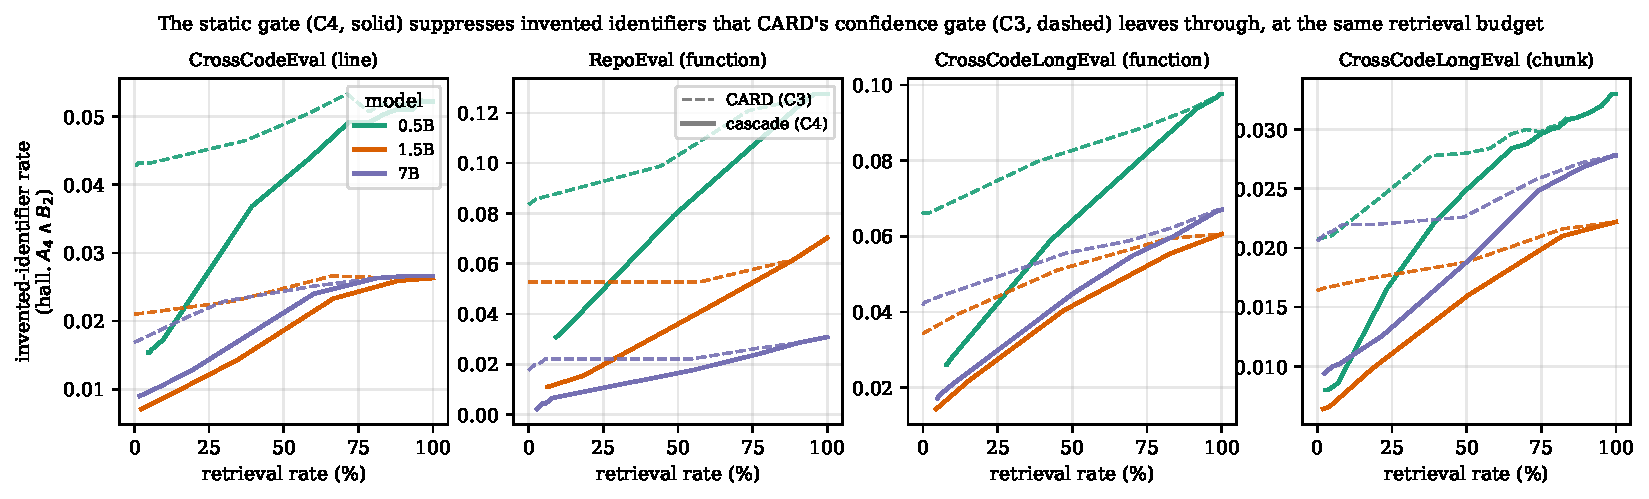
\includegraphics[width=\textwidth]{figures/fig_hallucination.pdf}
\caption{Invented-identifier rate vs.\ retrieval budget (RQ3). At a matched budget
the cascade (C4, solid) lies below CARD (C3, dashed) for every model; the gap is
largest at the low budgets where a selective policy operates, and closes as both
approach always-retrieve.}
\label{fig:hall}
\end{figure*}

\begin{figure*}[tb]
\centering
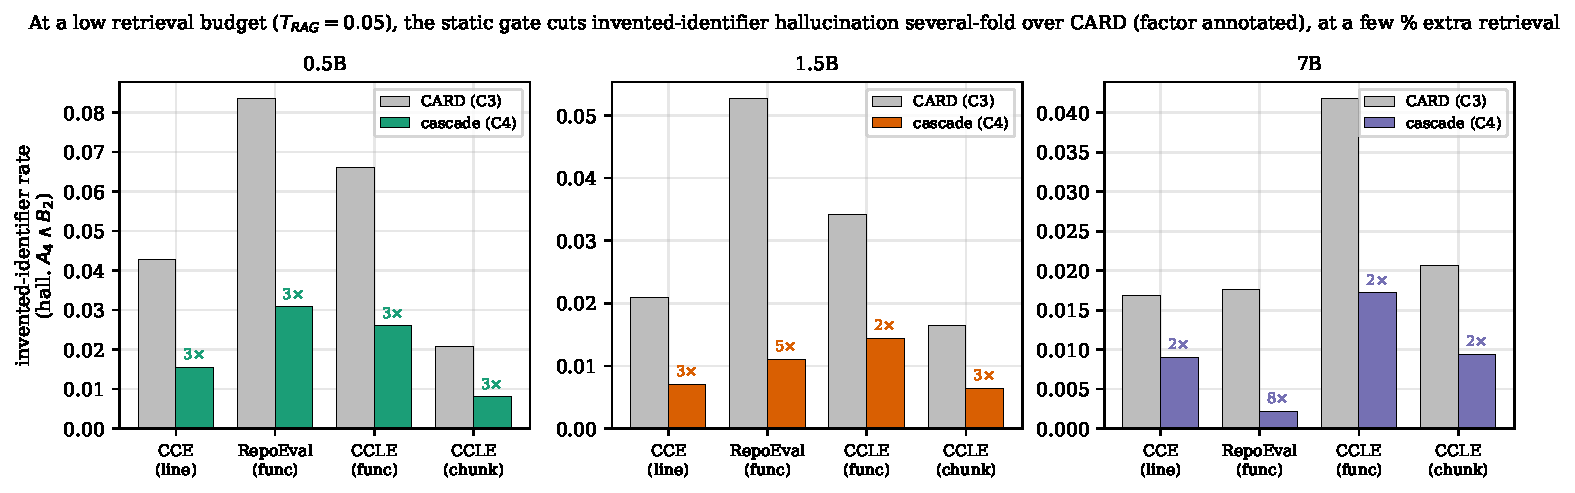
\includegraphics[width=\textwidth]{figures/fig_cascade_bars.pdf}
\caption{Headline reduction (RQ3): invented-identifier rate for CARD vs.\ the
cascade at $T_{\text{RAG}}=0.05$; the annotated factor is the reduction. The gate
is near-inert on the easy single-line control yet strongly beneficial on the
function tasks, exactly as hypothesised.}
\label{fig:cascade}
\end{figure*}

\subsection{RQ4: The gate is free and scales as hypothesised}
\textbf{No accuracy regression.} The cascade obeys an \emph{asymmetry guarantee} by
construction --- it only \emph{adds} retrieval to CARD's skip decisions --- and the
data confirm it empirically: at every one of the 19 thresholds, in every cell, C4
retrieval rate $\geq$ C3, C4 ES $\geq$ C3, and C4 $h_{A4B2}\leq$ C3
(Table~\ref{tab:cascade} shows ES ticking \emph{up}, e.g.\ CCLong-function 0.5B
$0.397\rightarrow0.424$). The hallucination reduction is thus obtained at no cost
to accuracy and only single-digit-percent extra retrieval (hence near-C1 latency).

\textbf{Scaling.} Accuracy rises monotonically with model size on every surface
(Table~\ref{tab:endpoints}). Invented-identifier rates fall with size on the
cleaner benchmarks (CCE C1 $h_{A4B2}$: $0.043/0.021/0.017$; RepoEval:
$0.084/0.053/0.018$ for 0.5B/1.5B/7B) but are noisier on the longer CCLong targets
(7B-function $0.042 \gtrsim$ 1.5B $0.034$) --- longer, harder contexts make even the
7B invent names, which is exactly where the gate keeps paying off. The contribution
is largest in absolute terms where hallucination is largest (smaller models,
function tasks) and is near-inert on the single-line control
(Fig.~\ref{fig:cascade}), as intended.

\textbf{Truncation matters.} Table~\ref{tab:dual} shows the headline (truncated)
ES is far above the raw ES on every multi-line surface (e.g.\ 7B CCLong-function C2
$0.839$ truncated vs.\ $0.426$ raw): without body/line truncation, over-generation
past the target span dominates the score. This both validates the truncation step
and underlines why the structural signal must be computed on the \emph{complete}
output rather than the truncated one (Section~\ref{sec:metrics}).

\begin{table}[tb]
\caption{RQ4 --- truncated (headline) vs.\ raw edit similarity. Over-generation
past the target span heavily deflates the raw score on every multi-line surface,
justifying span truncation for accuracy (and on-complete scoring for hallucination).}
\label{tab:dual}
\centering\footnotesize
\begin{tabular}{ll rr r rr}
\toprule
 & & \multicolumn{2}{c}{\textbf{C1 ES}} & & \multicolumn{2}{c}{\textbf{C2 ES}}\\
\cmidrule(lr){3-4}\cmidrule(lr){6-7}
Dataset & M & trunc. & raw & & trunc. & raw\\
\midrule
\multirow{3}{*}{RepoEval (func)} & 0.5B & 0.357 & 0.265 & & 0.717 & 0.475\\
 & 1.5B & 0.431 & 0.374 & & 0.887 & 0.615\\
 & 7B & 0.444 & 0.330 & & 0.839 & 0.444\\
\midrule
\multirow{3}{*}{CCLE (func)} & 0.5B & 0.397 & 0.287 & & 0.739 & 0.472\\
 & 1.5B & 0.468 & 0.389 & & 0.849 & 0.554\\
 & 7B & 0.489 & 0.356 & & 0.839 & 0.426\\
\midrule
\multirow{3}{*}{CCLE (chunk)} & 0.5B & 0.605 & 0.478 & & 0.846 & 0.564\\
 & 1.5B & 0.707 & 0.575 & & 0.935 & 0.681\\
 & 7B & 0.711 & 0.468 & & 0.924 & 0.511\\
\bottomrule
\end{tabular}
\end{table}


\section{Discussion}

\textbf{Confidence is not structure.} The adaptive-retrieval line of work gates on
the model's own uncertainty: FLARE~\cite{jiang2023flare} re-retrieves when the
next sentence contains low-probability tokens, and CARD~\cite{zhang2024card} trains
a critique model to predict the zero-shot output's edit similarity from logit
statistics. Our results make concrete a limitation implicit in both: token-level
confidence is necessary but not sufficient. A model can be perfectly confident in a
call to a helper that does not exist --- the tokens are individually likely because
the \emph{shape} is right --- and exactly these cases slip through the confidence
gate. The static check is cheap, training-free, and complementary: it reads the
same zero-shot output CARD already produced and asks an orthogonal question
(``does this resolve?'') rather than a confidence question (``is this likely?'').

\textbf{Retrieval is not a hallucination cure.} Repoformer~\cite{wu2024repoformer}
showed that always-retrieving is wasteful for \emph{accuracy} --- up to 80\% of
retrievals do not help. We add a sharper, complementary observation: always-retrieving
does not fix \emph{structural} hallucination and can worsen it
(Table~\ref{tab:endpoints}), because more context invites more (and longer)
generation, and thus more opportunities to invent names. This reframes selective
retrieval: the goal is not only to skip unhelpful retrievals but to \emph{spend the
budget on the structurally broken outputs}, which is exactly what the static gate
does. It also explains why the cascade's advantage is concentrated at low budgets
(Fig.~\ref{fig:hall}): once a policy retrieves almost everywhere, selectivity ---
and hence the gate's targeting --- has no room to act.

\textbf{Why functions.} The contribution tracks generation length: near-inert on
single-line CrossCodeEval, strongest on function bodies (Fig.~\ref{fig:cascade}).
This is intuitive --- a one-line completion rarely has space to call a non-existent
function --- and it is why benchmarks like CCLong~\cite{wu2024repoformer}, which
deliberately lengthen the target, are the right testbed for structural
hallucination. It also exposes a measurement subtlety the community should heed: a
model asked for one function over-generates into the next, so accuracy needs
span-truncation (Table~\ref{tab:dual}) \emph{while} the structural signal needs the
complete output; conflating the two (truncating before the static check) can
manufacture hallucinations that the model never produced.

\subsection{Implications}
For \textbf{practitioners}, the static gate is a near-zero-cost add-on to any
confidence-gated RAG completion system: it needs no training, runs in milliseconds
on the already-generated output, and removes the bulk of invented-identifier
hallucinations at a few percent extra retrieval and no accuracy loss --- a
favourable trade in an IDE setting where a confidently-wrong API call is more
damaging than a missing one. For the \textbf{research community}, our results argue
that (i) selective-retrieval policies should consider \emph{structural} signals,
not only confidence; (ii) repository-level completion should be evaluated with an
explicit structural-hallucination metric, not edit similarity alone, since
retrieval can improve ES while leaving (or worsening) hallucination; and (iii) such
metrics must be computed on the model's complete output, decoupled from the
accuracy-side truncation. The full per-instance results and the harness that
sweeps any gate over the budget axis are released to support this.

\subsection{Future Work}
\label{sec:future}
Several directions follow directly. First, \textbf{richer structural checks}: the
current gate flags an out-of-scope identifier (a scope/resolvability check);
extending it with signature/arity and import-origin checks could catch rarer but
higher-confidence structural errors that a pure scope check misses, at the cost of
consulting the cross-file symbol table. Second, \textbf{repair instead
of retrieve}: the static analyzer already localises the offending identifier, so a
cheaper action than full retrieval may be to constrain or correct that token.
Third, \textbf{better function-level critique labels}: Repoformer notes that
ES-based self-evaluation is miscalibrated for function completion, and our CARD
estimator inherits this; a structural or execution-based label could sharpen the
confidence gate so the cascade starts from a stronger base. Fourth,
\textbf{broader coverage}: more model families and sizes, and languages beyond
Python (the gate is language-agnostic in principle, needing only a parser and a
scope resolver). Finally, \textbf{repository-adaptive thresholds}, since duplication
and modularity vary across projects~\cite{zhang2023repocoder}.

\subsection{Threats to the Validity}
\textbf{Construct.} Edit similarity and exact match measure surface overlap, not
functional correctness; we do not run tests (pass@k), so a ``correct'' completion
may still be semantically wrong, and vice versa. Our hallucination metric is a
static proxy: pyflakes cannot resolve dynamically-created or star-imported names,
which could flag a valid identifier as undefined; we mitigate this by restricting
the gate to significant positions and by computing the signal on the reconstructed
file (which contains the in-file imports and definitions). There is a partial
\emph{circularity}: the cascade's trigger and the $h_{A4B2}$ metric both rest on
undefined-name analysis, so some of the measured reduction is structural by
construction; we address this by also reporting the independent absent-from-gold
rate $h_{A4}$ (which moves the same way) and by showing edit similarity never
decreases.

\textbf{Internal.} We re-implemented the CARD baseline rather than using original
code, and reused the 1.5B/7B critique estimators across datasets; a calibration
difference would shift C3 (and thus the C3$\rightarrow$C4 gap) but not the asymmetry
guarantee, which is structural. Generation is greedy and deterministic, so results
are reproducible but reflect a single decode. Latencies are measured under vLLM
continuous batching and are therefore throughput-amortised; we use them only for
within-benchmark, same-hardware comparison and rely on retrieval rate as the
hardware-independent cost proxy. We report point estimates over large test sets
(up to 5{,}000 instances); the harness supports paired McNemar and bootstrap tests,
which we leave to a camera-ready version.

\textbf{External.} Findings cover three code LMs (0.5B--7B), Python only, and four
benchmarks; larger models hallucinate less (Table~\ref{tab:endpoints}), so the
absolute benefit may shrink at frontier scale even as the asymmetry guarantee
persists. The CCLong-chunk surface strips blank lines during its construction,
which does not affect Python scoping but makes its raw text differ slightly from
on-disk source. Results on other languages or proprietary models may differ.

\section{Conclusion}
We set out to close a structural blind spot in adaptive retrieval for
repository-level code completion: confidence gates such as CARD skip retrieval on
outputs that are fluent but reference identifiers that exist nowhere in the
repository. Our remedy is a training-free static-analysis gate that runs only when
the confidence gate decides to skip, parses the zero-shot completion, and triggers
retrieval when it finds an out-of-scope identifier. Evaluated over four Python
surfaces and three code LMs (13{,}120 instances), with the retrieval budget swept
end to end, the cascade cuts the invented-identifier rate by $3.6$--$11\times$ over
CARD at a matched, single-digit-percent retrieval budget, never lowers edit
similarity (an asymmetry guarantee that holds at every threshold), and addresses a
failure mode that always-retrieving does not --- and sometimes worsens. The effect
is largest where it should be (smaller models, longer function targets) and
near-inert on easy single-line completions. Beyond the specific gate, the study
argues that selective retrieval should weigh \emph{structural} evidence alongside
confidence, and that repository-level completion should be measured with a
hallucination metric computed on the model's complete output. We release the code,
the full per-instance results, and the sweeping evaluation harness to make these
comparisons reproducible.



\bibliographystyle{IEEEtran}
\bibliography{main}



\newpage
\section{Appendix: Task Assignment Sheet}
\instruction{After discussion among yourself within your group, list the main project-related tasks assigned to and done by each team member. 
Tasks can be: conducting a literature review, preparing a dataset, implementation of technique X, code review, fine-tuning a model, prompt design, setting up eval pipeline, evaluating the technique X, improving repo documentation, writing section X of the report, preparing the presentation (section methodology, section evaluation, etc.).
The goal is to have a balanced task distribution among team members. }




% \begin{acks}
% You can thank people who helped you outside your group, e.g., if you had a user study you can thank the paeticipiants.
% \end{acks}


\end{document}